\chapter{Introducción}
\labch{intro}
\section{Cristalografía de rayos X}
\labsec{crx}
La cristalografía de rayos X es el método experimental más común para determinar la estructura de una (macro)molécula (\reftab{tab:pdb-stats}). En general, los modelos estructurales de las macromoléculas, obtenidos por medio de cualquier método experimental, se depositan en el banco de datos de proteínas (\acrshort{pdb}, por sus siglas en inglés) \sidecite[*-1]{Berman2000}. % El repositorio digital del \acrshort{pdb}, de libre acceso, se encuentra en el siguiente enlace \url{https://www.rcsb.org/}. 

\begin{table}[h]
	\centering
	\begin{tabular}{@{}llr@{}}
		\toprule
		Método experimental & Estructuras  & Porcentaje (\si{\percent})       \\ 
		\midrule
		Cristalografía de rayos X        & 153889 & 88.29 \\
		Resonancia magnética nuclear & 13195  & 7.57  \\
		Microscopía electrónica      & 6754   & 3.88  \\
		Difracción de neutrones	     & 177    & 0.10  \\
		Difracción de electrones     & 172    & 0.10  \\
		\midrule
		Suma                         & 174187 & 99.94 \\ \bottomrule
	\end{tabular}%
	\caption[Estructuras por método experimental]{Estructuras depositadas en el \acrshort{pdb} por método experimental-- Se listan los cinco métodos experimentales más usados en la determinación de estructuras macromoleculares. Datos actualizados al 06 de febrero del 2021. Fuente: \url{https://www.rcsb.org/}.}
	\labtab{tab:pdb-stats}
\end{table}

La cristalografía de rayos X, consiste en incidir rayos X sobre un cristal macromolecular. La energía de los rayos X se puede transferir a los electrones de las moléculas que conforman el cristal. Si la transferencia de energía se da de manera elástica, los electrones oscilaran con la misma frecuencia que la onda de rayos X incidente. Esto, según la electrodinámica clásica, resulta en una emisión de rayos X que a su vez pueden interferir entre sí, de forma destructiva o constructiva. Esta interferencia da lugar al concepto físico conocido como difracción. Si la diferencia entre las fases de las ondas de estos nuevos rayos X es exactamente igual a $n2\pi$ radianes, donde $n$ es un número entero, la interferencia será constructiva. Dada la naturaleza repetitiva del cristal, en general\sidenote{Existen ciertas condiciones de simetría que producen la extinción total de un punto de difracción.}, toda interferencia constructiva será amplificada y se podrá observar como un punto en el patrón de difracción (\reffig{fig:patron}).

El experimento de cristalografía de rayos X consiste en:

\begin{enumerate}
	\item Incidir rayos X sobre el cristal de la macromolécula de interés. 
	\item Obtener el patrón de difracción. 
	\item Rotar el cristal en cierto eje. 
	\item Repetir los pasos anteriores $n$ veces\sidenote{En general, $n$, depende de la simetría del cristal (véase la Tabla 1 de \cite{Dauter1999}).}.
\end{enumerate}

Cabe resaltar que si bien parece fácil, cada paso del experimento tiene dificultades inherentes y no es sencillo generalizar una colecta de datos porque esto depende del análisis final a realizar, de la configuración experimental y en gran manera, de la(s) macromolécula(s) estudiada(s). El objetivo del experimento es obtener una colecta de datos completa, es decir, obtener suficientes patrones de difracción para los pasos subsecuentes. El número de patrones de difracción es limitado y esto es causado por el daño por radiación.

\begin{figure}[hb]
	\includegraphics[width=0.9\textwidth]{imgs/patron}
	%Disponible en el siguiente enlace \url{tinyurl.com/ydfw6asv
	\caption[Patrón de difracción]{Patrón de difracción de la lisozima de clara de huevo de gallina.}
	%Los anillos concéntricos en el patrón de difracción, se denominan fajas de resolución. La resolución es el indicador principal de la calidad del modelo estructural de una proteína. Las fajas de alta/baja resolución corresponden a anillos más externos/internos.
	\labfig{fig:patron}
\end{figure}

\section{Daño por radiación}
\labsec{dpr}
\subsection{Introducción}
El daño por radiación se da porque los rayos X tienen la energía suficiente para ionizar la materia. Los electrones liberados provocan una serie de procesos químicos que resultan en la pérdida del orden cristalino. Esto significa que se pierde la amplificación en el proceso de difracción y en consecuencia los patrones de difracción cada vez contienen menos información. En otras palabras, la calidad del cristal decae y por lo tanto la calidad de cada patrón de difracción obtenido será cada vez menor. En consecuencia, cada cristal macromolecular presentará un límite temporal, denominado tiempo de vida útil, bajo el haz de rayos X. El daño por radiación es la principal causa de que sea difícil, o imposible, lograr el objetivo del experimento de la cristalografía de rayos X: obtener una colecta de datos completa.  
\subsection{Causa}
El daño por radiación se da porque los electrones de las moléculas que conforman el cristal, absorben la energía de los fotones incidentes. La absorción tiene su causa en uno de dos fenómenos físicos: el efecto fotoeléctrico o la dispersión inelástica. La probabilidad de que se dé el efecto fotoeléctrico es un orden de magnitud mayor que la dispersión inelástica, por lo que solo se describirá el primero. El efecto fotoeléctrico consiste en la absorción total de un fotón por un electrón. Como consecuencia el electrón es expulsado de su orbital dejando una vacante electrónica, o hueco positivo (\ce{h^+}), en la molécula que lo contenía. La energía de los electrones liberados, llamados fotoelectrones, se disipa en la trayectoria que estos hayan tomado; generando cientos\sidenote{El promedio de la primera energía de ionización para los átomos presentes, comúnmente, en una proteína es de \SI{12.67}{\electronvolt}; la energía de un fotón con una longitud de onda de \SI{1}{\angstrom} es de \SI{12398.4}{\electronvolt}.} de iones, radicales libres y eventos de excitación molecular. Los radicales son especies químicas que poseen uno o más electrones desapareados, por ende su reactividad es muy alta y su tiempo de vida es particularmente corto. Una reacción en cadena de radicales libres es inminente. Si algún radical, o cualquier especie química producto de la radiación, llegase a perturbar la red de contactos cristalinos, se pierde el orden cristalino. 
\subsection{Clasificación}
El daño por radiación se clasifica de acuerdo con su escala temporal. El daño primario es la ionización dada por el efecto fotoeléctrico. El daño secundario es la subsecuente cascada de radicales libres, dependiente del tiempo y de la temperatura. El daño terciario se define como el daño macroscópico sobre el cristal. Esto implica que una fracción suficiente de macromoléculas dentro del cristal ha sido afectada por el daño primario y secundario \sidecite{Teng2000}.
\subsection{Consecuencias}
Las consecuencias finales del daño por radiación están clasificadas en globales y específicas. En el primer apartado se tiene: (\emph{i}) la disminución de la intensidad de los puntos en el patrón de difracción, sobre todo aquellos en las fajas de alta resolución; (\emph{ii}) un cambio del volumen de la celda unitaria, lo que causa la pérdida de la isomorfía cristalina; (\emph{iii}) el aumento en los parámetros de desplazamiento atómico; y (\emph{iv}) el empeoramiento de las medidas que indican la calidad global de los datos \cite{Teng2000}. En el segundo apartado se tiene el daño específico, lo que significa cambios químicos puntuales en la estructura de la macromolécula cristalizada. Esto conlleva un orden dado: primero ocurre la reducción de átomos metálicos; después se da la ruptura de puentes disulfuro; luego la descarboxilación de aspartatos y glutamatos; y finalmente se pierde el grupo tiometilo de las metioninas \sidecite{Weik2000,Ravelli2000}. Residuos de aminoácido idénticos no son afectados de la misma manera, por ejemplo, no todas las metioninas son afectadas. Hasta el momento las razones de esto no han sido totalmente esclarecidas. Por este motivo, aunque existen ciertos principios básicos para determinar el daño específico, es difícil predecirlo y saber de antemano el grado en que afectará el modelo estructural obtenido. La relevancia de esto es inmensa, teniendo en cuenta que cerca del \SI{90}{\percent} de nuestro conocimiento de proteínas está dado por la cristalografía de rayos X. Por ejemplo, un modelo estructural incorrecto de una enzima, puede dar lugar a mecanismos de reacciones enzimáticas erróneos \sidecite{Matsui2002}.  %En el peor escenario, puede ser imposible obtener una estructura macromolecular debido a la inherente susceptibilidad del cristal al daño por radiación o a la pérdida de isomorfía cristalina.

\subsection{Métricas}
La mejor manera de determinar el daño por radiación en un cristal macromolecular, es estimando la dosis de radiación absorbida por el cristal. La dosis depende a su vez de la composición atómica del cristal y de algunos parámetros experimentales referentes al haz de rayos X \sidecite{Murray2004}. La dosis se mide en \si{\gray} que, según el Sistema Internacional de Unidades, es equivalente a la absorción de un Joule de energía ionizante por kilogramo de material irradiado. En experimentos de cristalografía de rayos X, es típico encontrar valores del orden de \si{\mega\gray} \sidecite{Garman2010}. Se han propuesto varias métricas para cuantificar el daño por radiación en función de la dosis absorbida; sin embargo, se ha demostrado que el uso de distintas métricas puede dar diferentes resultados \sidecite{Allan2013}. Actualmente no existe una métrica que haya sido acordada por unanimidad en el campo de la cristalografía de rayos X. 

El daño por radiación específico se puede visualizar (véase \reffig{fig:difden}). La manera de observalo es realizar colectas de datos idénticas y obtener la diferencia entre la densidad electrónica del modelo estructural de la colecta $n$, con cierta dosis de radiación absorbida y la colecta inicial, con una dosis de radiación absorbida mínima.

\begin{figure}[hb]
	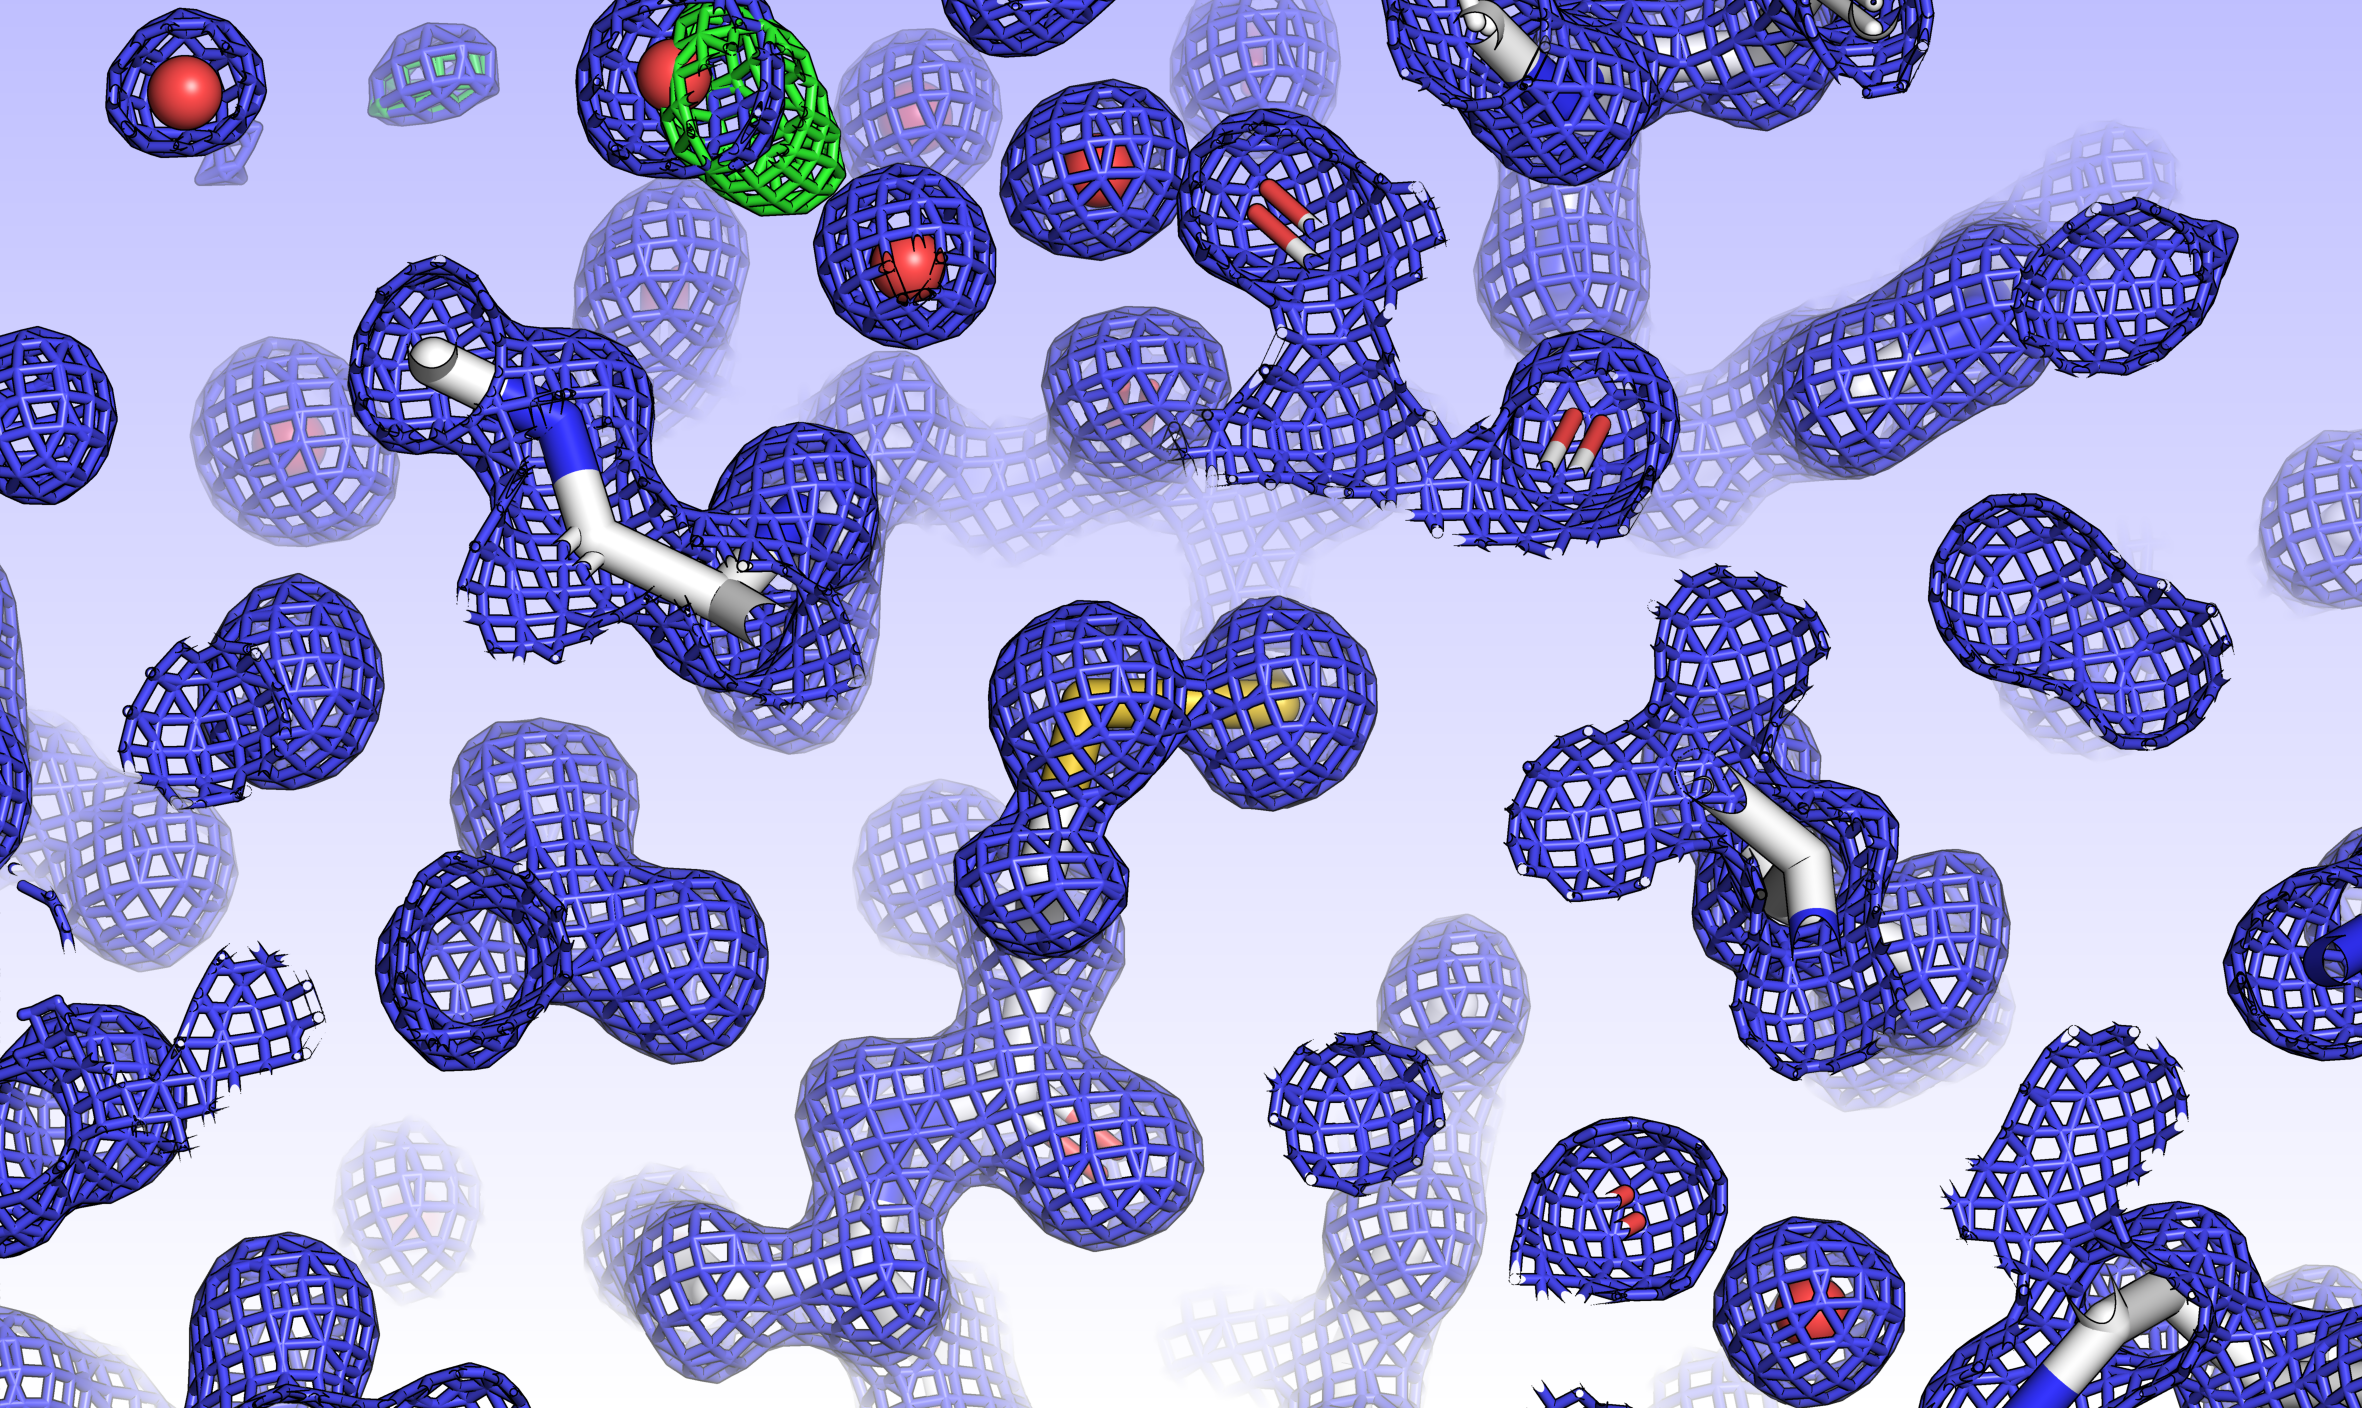
\includegraphics[width=0.75\textwidth]{imgs/before}
	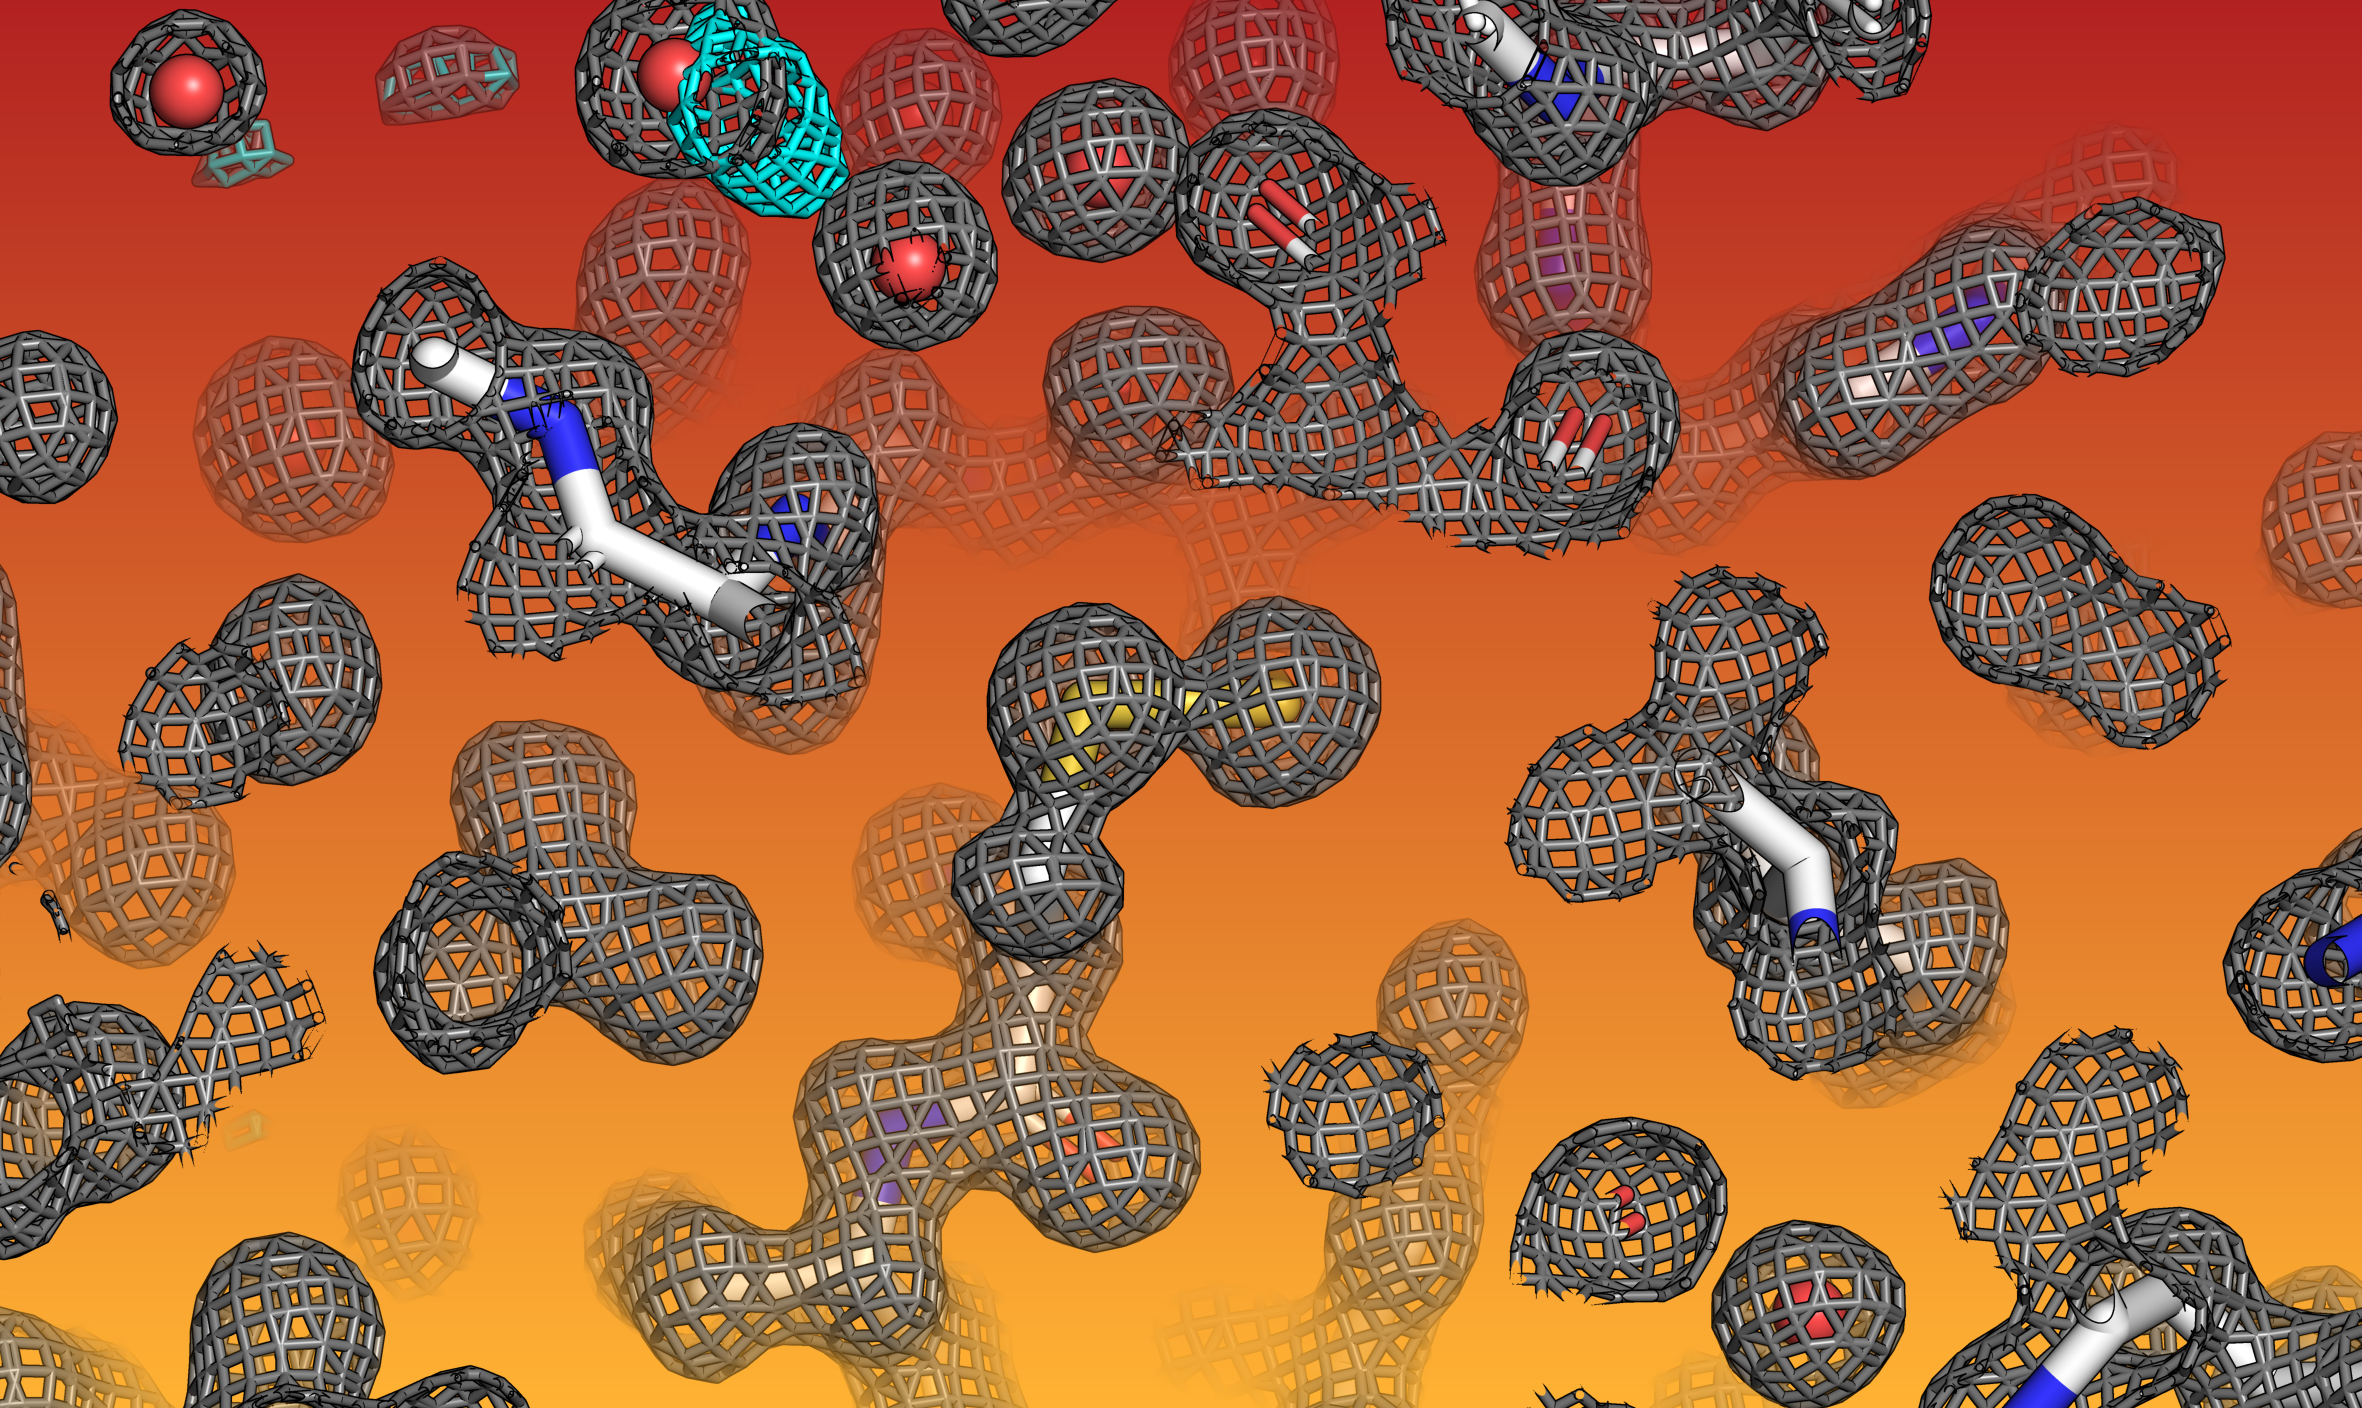
\includegraphics[width=0.75\textwidth]{imgs/after}
	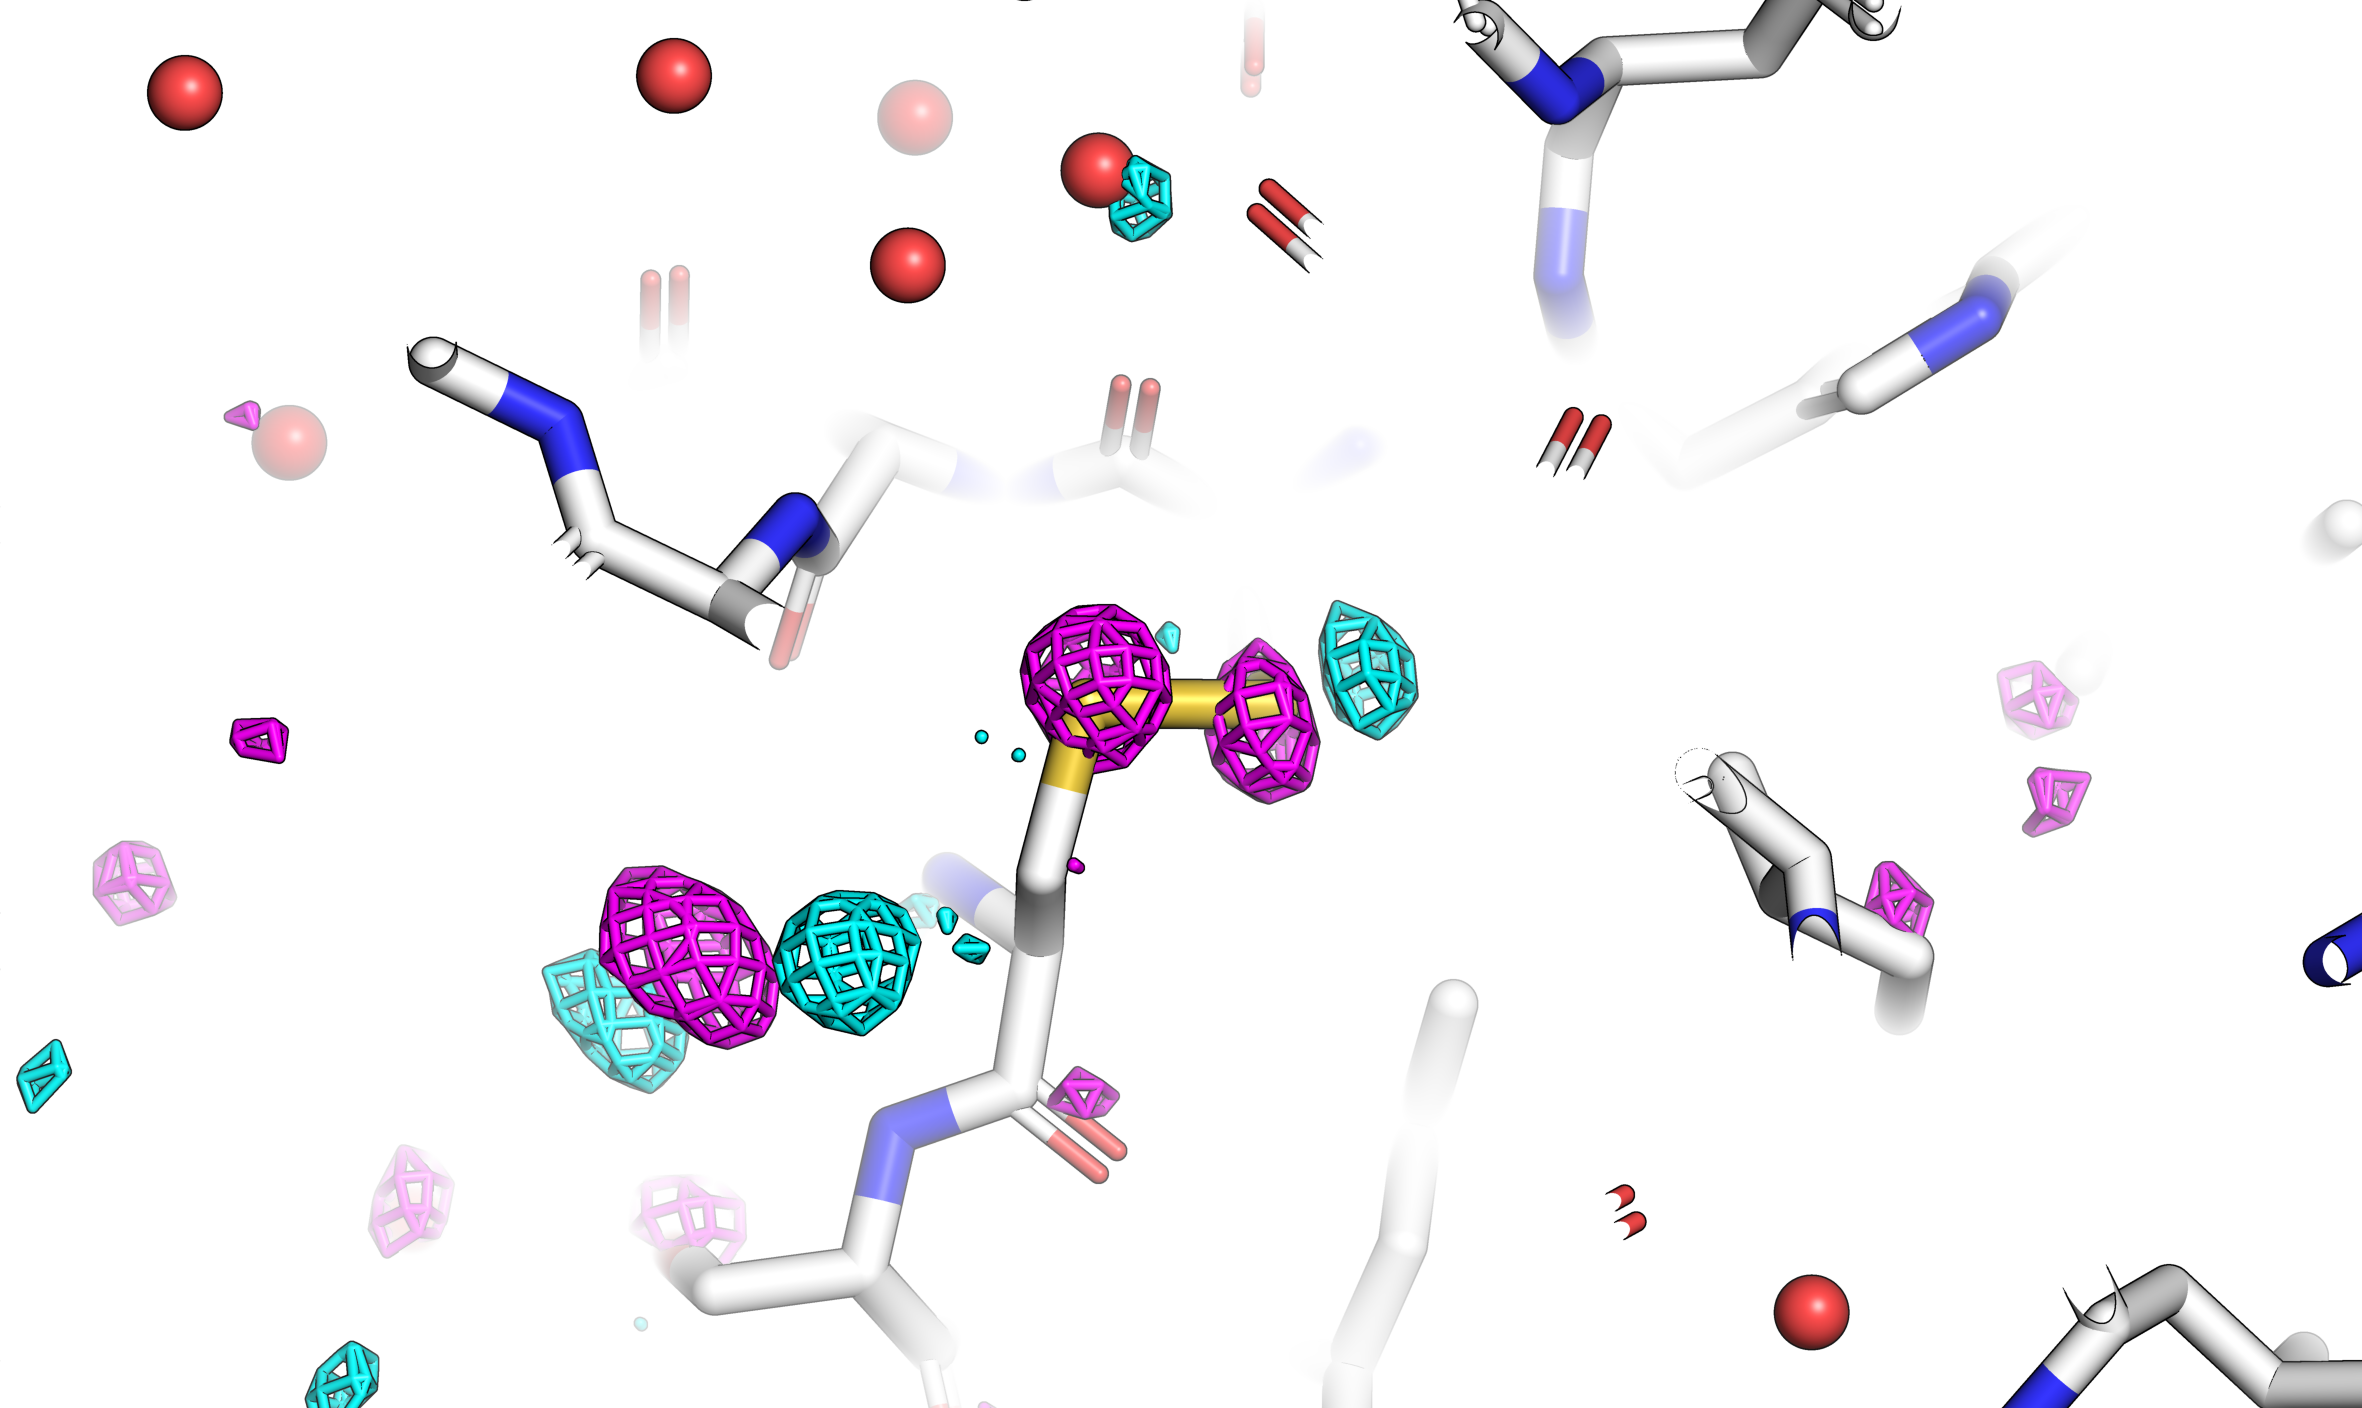
\includegraphics[width=0.75\textwidth]{imgs/diff}
	\caption[Diferencia de densidad electrónica]{Diferencia de densidad electrónica entre colectas de datos idénticas. Arriba: primer colecta de un cristal de lisozima (dosis absorbida \SI{0.6}{\mega\gray}). En medio: segunda colecta del mismo cristal (dosis absorbida \SI{3.2}{\mega\gray}). Los mapas $2F_{\mathrm{o}}-F_{\mathrm{c}}$ y $F_{\mathrm{o}}-F_{\mathrm{c}}$ se encuentran dibujados a \SI{1}{\sigma} y $\pm$\SI{3.5}{\sigma}, respectivamente. Abajo: La diferencia de densidad electrónica entre colectas $F_{\mathrm{o,2}}-F_{\mathrm{o,1}}$. Donde la diferencia negativa (magenta) está a \SI{-3.5}{\sigma} y la positiva (cian) a \SI{3.5}{\sigma}. Nótese como prácticamente no se observa una diferencia entre los mapas $2F_{\mathrm{o}}-F_{\mathrm{c}}$ (malla azul contra malla gris); sin embargo, sí existe una diferencia del modelo estructural inicial (el mismo en las tres imágenes) con respecto a la densidad electrónica de la segunda colecta. En otras palabras, para la segunda colecta, en una fracción de las proteínas cristalizadas este puente disulfuro se ha roto. Imagen realizada con PyMOL \cite{pymol} y datos de \cite{Nanao2005}. }
	\labfig{fig:difden}
\end{figure}


\section{Crioprotección}
\labsec{crio}
La primer estructura macromolecular determinada fue la de la mioglobina en 1958 por Kendrew y colaboradores \sidecite{Kendrew1958}. La forma de contender con el daño por radiación en aquella época era utilizando decenas de cristales y promediar los patrones de difracción. La regla de dedo para cambiar el cristal irradiado por uno nuevo, era seguir la intensidad de algunas reflexiones y si esta llegaba a disminuir de \num{20} a \SI{30}{\percent} de su valor inicial, entonces se procedía a reemplazar el cristal. 

El primer estudio en el que se valoró el potencial de la crioprotección, para reducir el daño por radiación, surgió por necesidad. Sucedía que ciertos cristales de insulina con átomos pesados sufrían un rápido desgaste por la radiación, en comparación con cristales de insulina sin átomos pesados. Con base en la observación de que el daño secundario es dependiente, en parte, de la temperatura; Low \emph{et al.} compararon, de manera cualitativa, el deterioro de los patrones de difracción colectados a \num{21}, \num{0} y a \SI{-13}{\celsius}. Los resultados fueron claros: a menor temperatura, mayor el tiempo de vida útil de los cristales  \sidecite{Low1966}. 

El problema con la reducción de temperatura en cristales macromoleculares, era la formación de hielo dentro de estos. Fue Haas quien primero usó crioprotectores para prevenir este problema. En el primer caso logró reducir la temperatura hasta \SI{-50}{\celsius}, remojando cristales de lisozima entrecruzados con glutaraldehído
en una mezcla de agua con glicerol \sidecite{Haas1968}. En un estudio posterior con cristales de lactato deshidrogenasa, el proceso de entrecruzamiento destruía los cristales. En cambio, si solo eran remojados por un par de días en una solución con sacarosa, el daño por radiación era diez veces menor \sidecite{Haas1970}. 
Es hasta 1988 que Hope describe por primera vez lo que conocemos hoy en día como criocristalografía de rayos X, donde básicamente se añade al cristal, o a la condición de cristalización, un crioprotector y el proceso de difracción del cristal se realiza a \SI{-173}{\celsius} \sidecite{Hope1988}. Una de las desventajas de esta técnica es encontrar las condiciones de crioprotección adecuadas para cada macromolécula. A pesar de este detalle, la crioprotección fue ganando adeptos de tal forma
que para el año 2000 era parte de la rutina de la \acrshort{drx} \sidecite{Garman2003}. Gracias a la crioprotección, en general era suficiente un único cristal macromolecular para obtener un
\enquote{dataset} completo.

\section{Sincrotrones}
\labsec{sincro}
La principales fuente de rayos X para realizar el experimento de \acrshort{drx}, es la radiación sincrotrón.
La historia tecnológica de los sincrotrones se divide en generaciones. La primera generación de sincrotrones eran aquellos pertenecientes al campo de la física de partículas, donde los primeros estudios con respecto a la estructura de proteínas fueron realizados \sidecite{Phillips1976}. Para la década de 1980 se construyen los sincrotrones dedicados a la biología estructural, esta es la segunda generación. Para la década de 1990 llega la tercera generación. El primer sincrotrón perteneciente a la cuarta generación empezó a operar en 2016 \sidecite{Owen2016}. 
Una de las características de un sincrotrón es su brillo espectral, que se define como la distribución del flujo de fotones en el espacio y el rango angular. El flujo se establece como el número de fotones por segundo que atraviesan un área definida por un ancho de banda dado \sidecite{Willmott2019}. La revolución tecnológica de los sincrotrones se nota en la diferencia del orden de magnitud del brillo espectral \cite{Willmott2019}. Este aumento en brillo se ha permitido pues permite una gran ventaja: la posibilidad de utilizar cristales de menor tamaño. Esto es porque la principal limitante de la \acrshort{drx} es obtener cristales macromoleculares, en particular cristales de un tamaño adecuado (al menos unos cien micrómetros en sus tres dimensiones\sidenote{Existen líneas especiales donde existe la posibilidad de usar cristales con un orden de magnitud menor, las denominadas líneas microfoco.}.) 

Actualmente se está desarrollando la tecnología para cambiar la metodología de la colecta de datos, usando cristales macromoleculares nanométricos y con una fuente de rayos X más poderosa denominada \acrshort{xfel} (del inglés \emph{X-ray Free Electron Laser}). Existen ya varios estudios en los que se ha demostrado la posibilidad de obtener estructuras macromoleculares con esta nueva metodología \sidecite{Martin-Garcia2016}. Sin embargo, el acceso al tiempo experimental en un XFEL es actualmente muy limitado.

Como se mencionó en la sección anterior, ya para el año 2000, la noción general en el campo de la criocristalografía era que el daño por radiación era insignificante, un problema del pasado. Precisamente esta noción cambia en ese mismo año, cuando tres estudios independientes muestran el efecto del daño por radiación en la entonces nueva generación de sincrotrones \sidecite{Teng2000,Weik2000,Ravelli2000}. 

\section{Radioprotectores}
\labsec{radio}
Al ser evidente que el daño por radiación aumentaba con el incremento en brillo, fue necesario buscar estrategias, como la crioprotección, que ayudaran a mitigar el daño por radiación. En el curso de los últimos veinte años, se han investigado varias estrategias pre y posteriores a la difracción con distintos enfoques \sidecite{Garman2017}. Una de las tantas estrategias, es el uso de moléculas pequeñas que interactuan con los radicales libres generados por la radiación. Estas moléculas se denominan radioprotectores. Sin embargo, en la literatura científica existen varias incongruencias con respecto a la efectividad de los radioprotectores y es por esto que la comunidad cristalográfica no ha adoptado al cien por ciento el uso de radioprotectores de manera rutinaria \sidecite{Nowak2009, Allan2013}.
